\chapter{Evaluation}\label{chap:Evaluation}
This section evaluates how successfully and effectively the implemented features achieve the goals stated in the introduction.

\section{Success}
This evaluation is more ambitious than that presented in the project proposal goals. As demonstrated below, the type witness search procedure and cast slicing features exceeds all core goals\footnote{That is, reasonable coverage and performance.} presented in the project proposal, while type slicing had not been conceived, but naturally complements cast slicing. Some extension goals were reached: almost of Hazel was supported\footnote{Except the type slicing of two constructs: type functions and labelled tuples (which was a new feature merged by the Hazel dev team in February).}. The search procedure was not mathematically formalised, but the slicing mechanisms were.

\section{Goals}\label{sec:EvaluationGoals}
This project devised and implemented three features: \textit{type slicing, cast slicing,} and a \textit{static type error witness search procedure}. Each of which had a clear intention for it's use:

\paragraph{Type Slicing:} Expected to give a greater static context to expressions. Explaining why an expression was given a specific type.

\paragraph{Cast Slicing:} Expected to provide static context to runtime type casts and propagate this throughout evaluation. Explaining where a cast originated and why it was inserted.

\paragraph{Search Procedure:} Finds dynamic type errors (cast errors) automatically, linked back to source code by their execution trace and \textit{cast slice}. Therefore, a static type error can be associated automatically with a concrete dynamic type error \textit{witness} to better explain.

\section{Methodology}\label{sec:EvaluationMethodology}
I evaluate the features and their various implementations (where applicable) along \textit{four} axes. With quantitative measures were evaluated over a corpus of ill-typed and dynamically-typed Hazel programs (\cref{sec:CorpusCollection}):

\subsubsection{Quantitative Analysis}
\paragraph{Performance: } \textit{Are the features performant enough for use in interactive debugging? Which implementations perform best?}

The time and space usage of the search procedure implementations were micro-benchmarked for each ill-typed program in the corpus. Up to 100 runs were taken per program with estimated time, major and minor heap allocations were estimated using an ordinary linear regression (OLS) via the \textit{bechamel} library \cite{Bechamel}.

\paragraph{Effectiveness: } \textit{Do the features effectively solve the problems? Are the results easily interpretable by a user?}

The \textit{coverage},  what proportion of programs admit a witness, for each search procedure implementation was measured. The search procedure does not always terminate, a 30s time limit was chosen. The coverage was expected to be \textit{reasonable}, chosen at 75\%.

Additionally, the \textit{size} of witnesses, evaluation traces, type slices, and cast slices were measured. The intention being that a smaller size implies that there is less information for a user to parse, and hence easier to interpret.\footnote{Not necessarily \textit{always} true, but a reasonable assumption.}

\subsubsection{Qualitative Analysis}
\paragraph{Critical: } \textit{What \textit{classes} of programs are missed by the search procedure? What are the implications of the \textit{quantitative} results? What improvements were, or could be made in response to these?}

This section provides \textit{critical} arguments on {usefulness} or {effectiveness}, which are \textit{evidenced} by quantitative data. Differing implementations and \textit{subsequent improvements}\footnote{Which were then implemented and analysed.} are compared. Additionally, further unimplemented improvements are proposed.

\paragraph{Holistic: } \textit{Do the features work well together to provide a helpful debugging experience? Is the user interface intuitive?}

Various program examples are given, demonstrating how all three features can be used together to debug a type error. Improvements to the UI are discussed.\footnote{Improved UI being a low-priority extension.} 



\section{Hypotheses}
Various hypotheses for properties of the results are expected. The evidence and implications of these are discussed in the \textit{critical evaluation}.

\paragraph{Search method space requirements: } The space requirements for DFS and Bounded DFS are expected to be lower than that of BFS and interleaved DFS.

\paragraph{Type Slices are larger than Cast Slices: } Casts are de-constructed during elaboration and evaluation, so cast slices are expected to be smaller than the original type slices, and therefore more directly explain why errors occur. 

\paragraph{The Small Scope Hypothesis: }
\label{sec:SmallScopeHypothesis} This hypothesis \cite{SmallScopeHypothesisOrigination} states that a high proportion of errors can be found by generating only \textit{small} inputs. Evidence that this hypothesis holds has been provided for Java data-structures \cite{SmallScopeHypothesis} and answer-set programs \cite{SmallScopeHypothesisAnswerSet}. Does it also hold for finding dynamic type errors from small \textit{hole instantiations}?

\paragraph{Smaller instantiations correlate with smaller traces: } As functional programs are often written recursively, destructuring compound data types on each step. If this and the small scope hypothesis hold, then most errors could be found with \textit{small execution traces}.

\section{Program Corpus Collection}\label{sec:CorpusCollection}

A corpus of small and mostly ill-typed programs was produced, containing both dynamic (unannotated) programs and annotated programs (containing statically caught errors). We have made this corpus available on GitHub \cite{HazelCorpus}.

\subsection{Methodology}
There are no extensive existing corpora of Hazel programs, nor ill-typed Hazel programs. Therefore, we opted to transpile parts of an existing OCaml corpus collected by Seidel and Jhala \cite{OCamlCorpus}. Which is freely available under a Creative Commons CC0 licence. 

I am grateful for my supervisor who created a best-effort OCaml to Hazel transpiler \cite{HazelOfOCaml}. This translates the OCaml examples into both a dynamic example, and a (possibly partially) statically typed version according to what type the OCaml type checker expects expression to be.\footnote{The annotations may be consistent, as we are translating ill-typed code.}

This corpus contains both OCaml unification and constructor errors. When translated to Hazel, these may manifest as differing errors. The only errors that the search procedure is expected to detect are those which contain \textit{inconsistent expectations} errors. Hence, the search procedure is ran on the corpus of annotated programs filtering those without this class of errors. Additionally, the search procedure requires the erroneous functions to have holes applied to start the search, these are inserted automatically by the evaluation code after type checking the programs.


\subsection{Statistics}
The program corpus contains \textbf{698} programs of which \textbf{203} were applicable to performing the search procedure on. Averages and standard deviations in size and trace size\footnote{When using normal, deterministic, evaluation.} shown in \cref{fig:CorpusStats}.
\begin{figure}
\centering
\begin{tabular}{c|ccccc}
& \textbf{Count} & \multicolumn{2}{c}{\textbf{Prog. Size}}& \multicolumn{2}{c}{\textbf{Trace Length}}\\
&  & Avg. & Std. dev. & Avg. & Std. dev.\\
\hline
\textbf{Unannotated} &404 &117 &81 &9&9\\
\textbf{Annotated} &294 &117 &76 &9&9\\
\textbf{Searched} &203 &120 &77 &10 &10\\
\hline
(Total)  &698 &117 &79 &9 &9\\
\end{tabular}
\caption{Hazel Program Corpus}
\label{fig:CorpusStats}
\end{figure}

\section{Performance Analysis}\label{sec:PerformanceAnalysis}

\subsection{Slicing}
The type and cast slicing mechanisms don't increase the time complexity of the type checker nor evaluator. Hence, they are still as performant as the original, capable of interactive use to medium sized programs.

\subsection{Search Procedure}
Only the annotated ill-typed corpus containing inconsistency errors are used in evaluating the search procedure. After all, any well-typed program cannot have a dynamic type error.

As the search procedure may be non-terminating, these results are found given a 30s time limit. Micro-benchmarking the programs which do not time-out, the time and space used searching for each witness can be estimated. The averages over all successful programs for each implementation are given in \cref{fig:SearchPerformance}. These results suggest that, as expected, BFS and interleaved DFS (IDFS) use more memory in total\footnote{Although, IDFS efficiently keeps most memory allocated short lived, being in the \textit{minor} heap.} than bounded DFS (BDFS) and DFS, while DFS is the fastest\footnote{Having the least overhead.}. 

However, full averages are not a fair test as the sets of programs averaged over are different, for example, BFS only happens to succeed on the smaller programs. Hence, the ratios between each implementation as compared to DFS on only the programs which \textit{both} succeed on are given in \cref{fig:SearchPerformanceRatios}. Under this, the results are even more pronounced.
\begin{figure}
  \centering
  \begin{tabular}{lc|cccc}
  & Averages & \multicolumn{4}{c}{\textbf{Implementations}}\\
   & unit & \texttt{DFS} & \texttt{BDFS} & \texttt{IDFS} & \texttt{BFS}\\
   \hline
   \textbf{Time} & ms &  7.6 & 73 & 140 & 120\\
   \textbf{Major Heap} & mB & 3.7 & 32 & 5.9 & 25\\
   \textbf{Minor Heap} & mB & 66 & 680 & 1900 & 1300
  \end{tabular}
  
\caption{Benchmarks: Search Implementations}
\label{fig:SearchPerformance}
\end{figure}
\begin{figure}
  \centering
  \begin{tabular}{l|ccc}
  Ratios & \multicolumn{3}{c}{\textbf{Implementations}}\\
    vs. \texttt{DFS}& \texttt{BDFS} & \texttt{IDFS} & \texttt{BFS} \\
   \hline
   \textbf{Time} &  8.3 & 52 & 230\\
   \textbf{Major Heap} & 9.0 & 3.2 & 270\\
   \textbf{Minor Heap} & 9.7 & 83 & 390
  \end{tabular}
  
\caption{Benchmarks: Performance ratios to DFS over common programs}
\label{fig:SearchPerformanceRatios}
\end{figure}


\section{Effectiveness Analysis}\label{sec:EffectivenessAnalysis}


\subsection{Slicing}
\textit{Type slice} sizes were calculated by the type checker over the entire corpus, where the size is the number of constructs highlighted. While \textit{cast slice} sizes were calculated over in the elaborated expressions after type checking.

\Cref{fig:TypeSlicingEffectiveness} shows that both type and cast slices are generally small. In particular, the proportion of the context\footnote{Calculated by close approximation by the \textit{program size}. As each program in the corpus is just one definition. Calculating the context itself is non-trivial.} highlighted is very low, generally less than 5\% for dynamic code and 10\% for annotated code. Therefore, they concisely explain the types. However, some slices are still large, as seen by the relatively large standard deviations.

Additionally, for errors, there will be multiple inconsistent slices involved. \Cref{sec:SlicingAnalysis} describes how these slices can be summarised to only report the inconsistent parts. We find that these \textit{minimised} error slices are significantly (3x) smaller than directly \textit{combining} the slices.

\begin{figure}[h]
  \centering
  \begin{tabular}{lc|c|ccc|ccc}
  \multicolumn{2}{c}{\textbf{Averages}} & \multicolumn{7}{c}{\textbf{Subdivisions}}\\
  & & & \multicolumn{3}{c|}{\textbf{Combined Error Slices}} & \multicolumn{3}{c}{\textbf{Minimised Error Slices}}\\ 
   & unit & ok & expects & branches & all & expects & branches & all\\
   \hline
   \textbf{Type Slice} & size &  8.2 & 13 & 22 & 15&  5.7 & 3.2 & 5 \\
   Std. dev. &  				 &  11 & 10 & 24 & 15&    4.31 & 4.1 & 4.4 \\
   \textbf{Proportion}& \%    & 5 & 8 & 14 & 9&        3  & 2 & 3 \\
   Std. dev. &  				 &  7 & 8 & 14 & 10&      3 & 3 & 3 \\
   \multicolumn{9}{c}{\textit{(Unannotated)}}\\
   \textbf{Type Slice} & size &  7.5 & 21 & 133* & 22.6 &8.2&  2.0* & 8.2  \\
   Std. dev. 			&    &  13 & 22 & 42* & 25.2& 12.6&  0.0* & 12.6  \\
   \textbf{Proportion}& \% 	 & 4 & 14 & 0.48* & 15&  6&    1* & 5  \\
   Std. dev. &  				 &  9 & 18 & 0.07* & 18&   9&    0* & 12  \\
   \multicolumn{9}{c}{\textit{(Annotated)}}\\
   \multicolumn{9}{c}{* only 2 annotated programs had inconsistent branches}
  \end{tabular}
  \caption{Effectiveness: Type Slices}
\label{fig:TypeSlicingEffectiveness}
\end{figure}
Casts have a pair of slices, \textit{`from'} a type and \textit{`to'} a type. As hypothesised, both of which are smaller on average (\cref{fig:CastSlicingEffectiveness}) than type slices. Therefore, casts can more precisely point to which part of an expressions type caused them.

Unnanotated code has larger \textit{`from'} slices as it relies more on synthesis for typing code, and vice versa for annotated code.



\begin{figure}[h]
  \centering
  \begin{tabular}{lc|cc|cc}
  \multicolumn{2}{c}{\textbf{Averages}} & \multicolumn{4}{c}{\textbf{Subdivisions}}\\
  & & \multicolumn{2}{c|}{\textbf{Ok}} & \multicolumn{2}{c}{\textbf{Errors}}\\ 
   & unit & from & to & from & to\\
   \hline
   \textbf{Cast Slice} & size &  5.5 & 1.2 & 5.9 & 1.5 \\
   Std. dev. &  				 &  8.1 & 3.7 & 7.1 & 2.0\\
   \textbf{Proportion}& \%    & 1 & 0.2 & 1 & 0.2\\
   Std. dev. &  				 &  1 & 0.5 & 1 & 0.4\\
   \multicolumn{6}{c}{\textit{(Unannotated)}}\\
   \textbf{Type Slice} & size &  4.8 & 6.3 & 6.9 & 4.4  \\
   Std. dev. 			&    &  11 & 13 & 9.1 & 9.3\\
   \textbf{Proportion}& \% 	 & 1 & 2 & 2 & 1\\
   Std. dev. &  				 &  1 & 1 & 1 & 1\\
   \multicolumn{6}{c}{\textit{(Annotated)}}
  \end{tabular}
  \caption{Effectiveness: Cast Slices}
\label{fig:CastSlicingEffectiveness}
\end{figure}


\subsection{Search Procedure}

\subsubsection{Witness Coverage}
\begin{figure}[h]
\centering
\begin{subfigure}{0.45\textwidth}
\centering
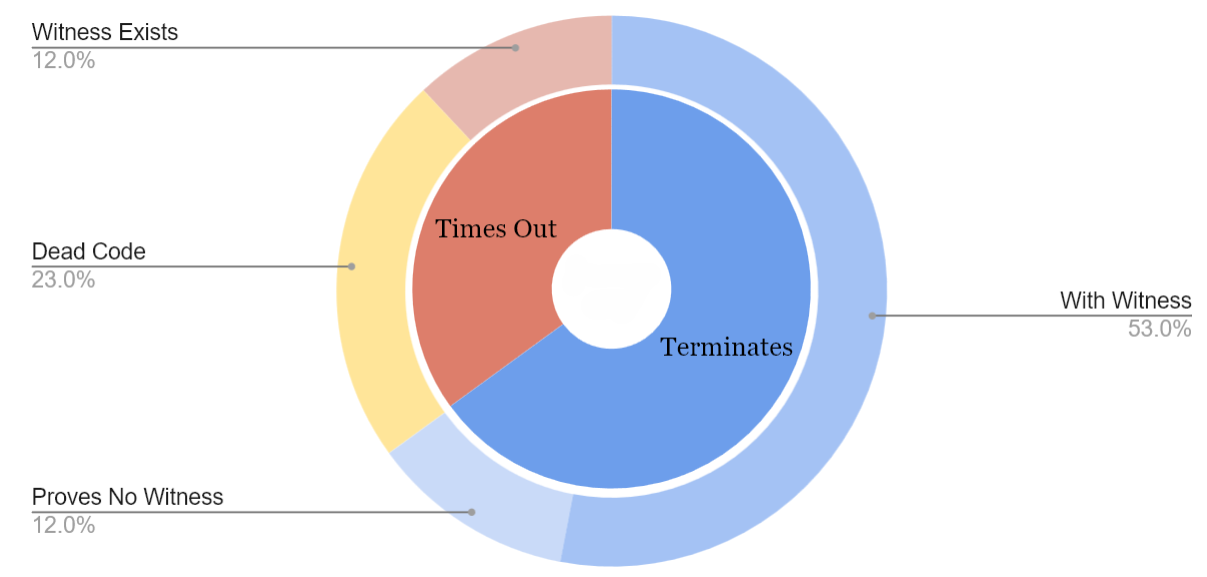
\includegraphics[width=1\textwidth]{Media/Figures/DFS_coverage}
\caption{DFS}
\end{subfigure}
%
\begin{subfigure}{0.45\textwidth}
\centering
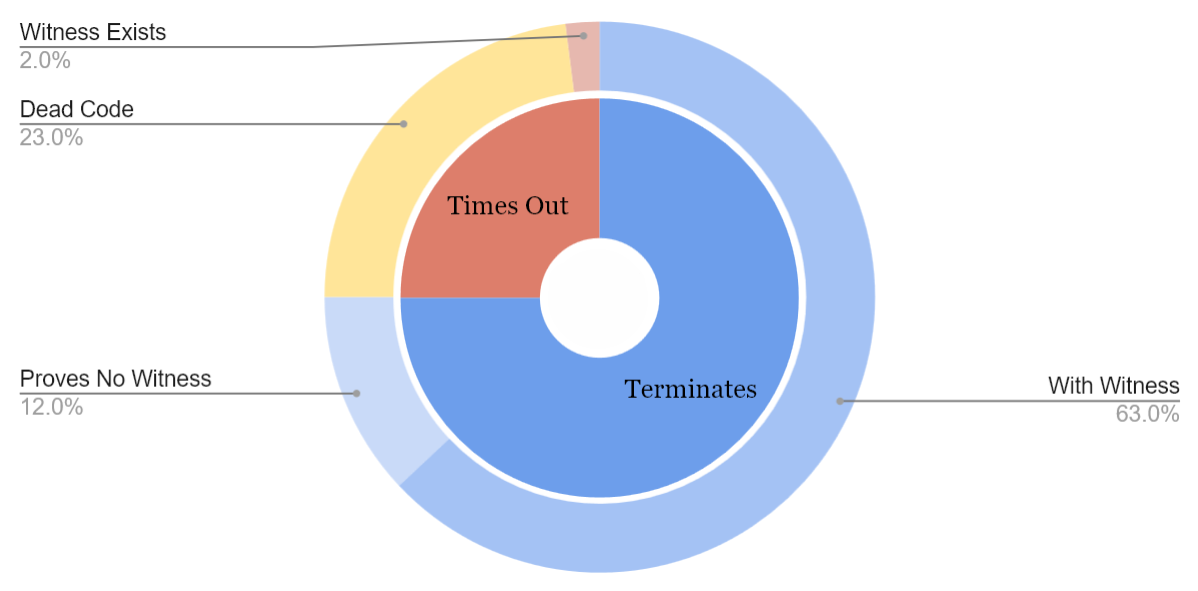
\includegraphics[width=1\textwidth]{Media/Figures/BDFS_coverage}
\caption{Bounded DFS}
\end{subfigure}

\vspace{1cm}

\begin{subfigure}{0.45\textwidth}
\centering

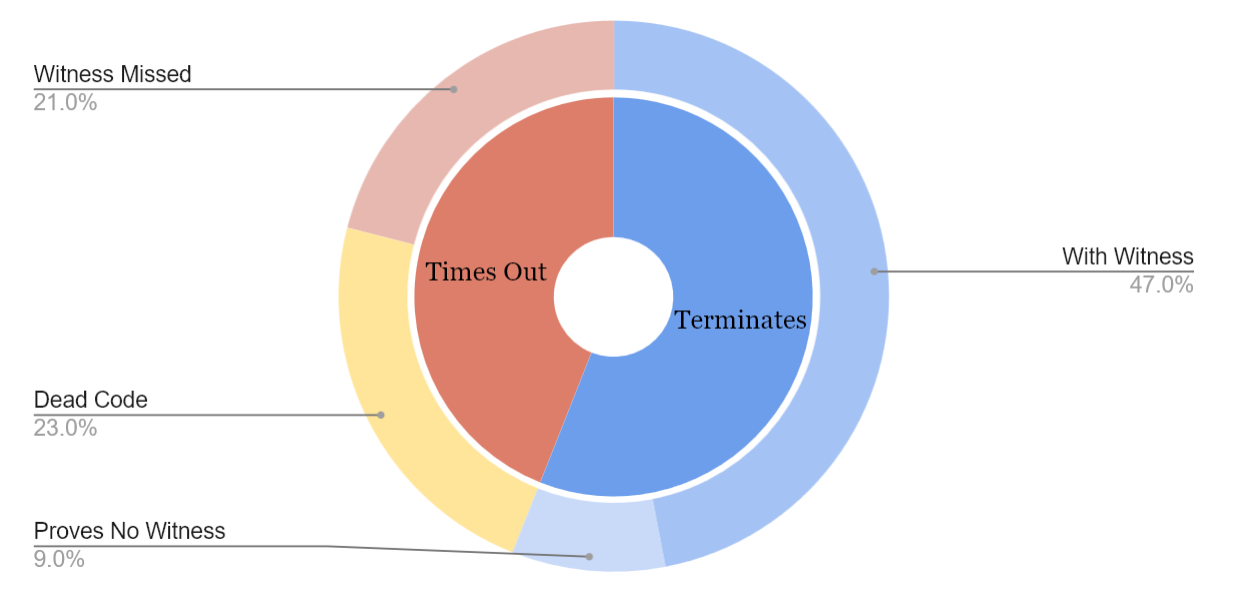
\includegraphics[width=1\textwidth]{Media/Figures/IDFS_coverage}
\caption{Interleaved DFS}
\end{subfigure}
%
\begin{subfigure}{0.45\textwidth}
\centering

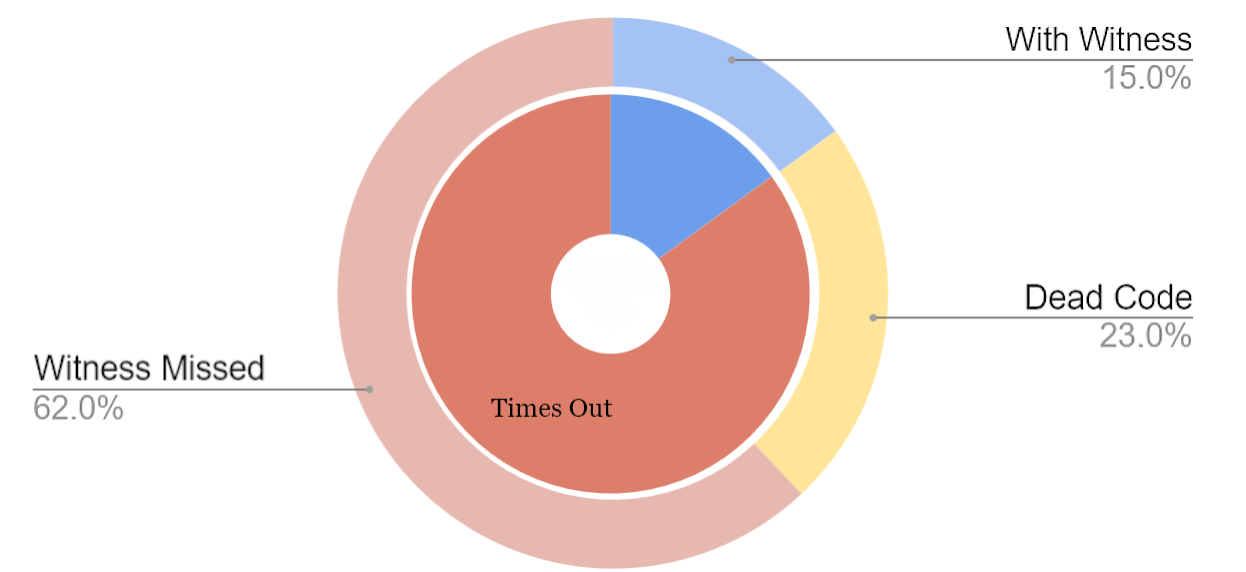
\includegraphics[width=\textwidth]{Media/Figures/BFS_coverage}
\caption{BFS}
\end{subfigure}

\caption{Search Procedure Coverage}
\label{fig:PieChart}
\end{figure}

The search procedure terminates either with a witness or proving no witness exists. A majority of programs terminated when using BDFS, DFS and IDFS, with BDFS meeting the 75\% target directly (\cref{fig:PieChart}). IDFS and BFS perform relatively poorly likely due to excessive memory usage (\cref{fig:SearchPerformance}). 

However, not all programs actually have an execution path leading to a dynamic type error. For example, errors within dead code cannot be found. I manually classified each failed program for BDFS to check if a witness does exist, but was not found, or no witness exists. Of which, 89\% was found to be dead code and 5\% due to Hazel bugs\footnote{Being also present on the main branch, not just in my code.}; the bugs were excluded from the results. This gives only 2\% of cases where BDFS failed to actually find an \textit{existing} witness; DFS and IDFS also meet the goal of failing in less than 25\% of cases. \Cref{sec:SearchCategories} goes into further detail on categorising the programs which time out, and how this could be avoided.

\subsubsection{Witness \& Trace Size}
As predicted by the small-scope hypothesis, most programs admitted \textit{small} witnesses. And the depth first searches produce longer and more varied trace lengths, which allowed them, in combination with their lower memory overhead, to attain higher coverage (many witnesses were at a deeper depth than IDFS or BFS were able to reach).

However, there was no linear correlation (Pearson correlation coefficient $= 0$) between witness sizes and trace sizes, even when normalised by the original deterministic evaluation trace lengths. This is likely because most errors are in the base cases, so few large witnesses are even found, with the noise from trace lengths to different programs' base cases dominating. 

\begin{figure}[h]\centering
\begin{tabular}{l|cccc}
& DFS & BDFS & BFS & IDFS\\
\hline
\textbf{Witness Size} Avg. & 1.1& 1.9&1.4&  2\\
Std. dev. & 1.2& 2.3&1.4&  2.3\\
\textbf{Trace size} Avg. & 33& 32& 11& 17\\
Std. dev. & 35& 33&2.4& 5
\end{tabular}
\caption{Witness \& Trace Sizes}
\label{fig:WitnessSize}
\end{figure}


\section{Critical Analysis}\label{sec:CriticalAnalysis}
This section discusses the implications of the previous results and delves deeper into the reasoning behind them. As a response to this analysis, many improvements have been devised, some of which have been implemented.
\subsection{Slicing}\label{sec:SlicingAnalysis}
Contribution slicing often highlights large, verbose slices, including many irrelevant branches, mostly justifying subsumption in subterms, which never relates directly to type errors. Therefore, we use synthesis and analysis slices to explain static errors more concisely. Users can still select subterms to inspect their type consistency if needed.

Type slicing theory (\cref{sec:TypeSlicingTheory}) requires highlighted code to form valid expressions or contexts, though some highlighted parts, like unused or dynamic bindings, don't affect types and can be omitted. This motivated the use of unstructured (ad-hoc) slices (\cref{sec:UnstructuredCodeSlice}).

In \cref{fig:LetSliceOmitted}, a bound integer \code{x} is only used in one branch. Since the other branch can already determine the type of the conditional, the $\code{x}$  and \code{let} are excluded from the slice. Though the whole program is selected,\footnote{See the red cursor.} the let expression is omitted. A contribution slice would include everything,\footnote{Both branches must be shown, as \code{x} needs to type-check.} making it even more verbose.
\begin{figure}
\centering
\begin{subfigure}{0.45\textwidth}
\centering

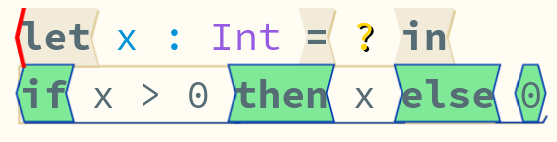
\includegraphics[width=0.85\textwidth]{Media/Figures/Unused_let}
\caption{Ad-hoc Slice: Let expression omitted}
\end{subfigure}$\qquad$
\begin{subfigure}{0.45\textwidth}
\centering

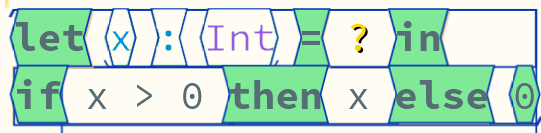
\includegraphics[width=0.85\textwidth]{Media/Figures/Unused_let_ordinary}
\caption{Ordinary Slice}
\end{subfigure}

\caption{An Ad-hoc Slice vs. Ordinary Slice}
\label{fig:LetSliceOmitted}
\end{figure}


\subsubsection{Error Slices}
\label{sec:ErrorSlices}
Type errors arise from inconsistencies between a term’s analysis and synthesis slices, or across synthesising branches. Understanding the error requires comparing all the slices involved.

Some type parts may agree, hence another form of type joining was introduced to isolate only the inconsistent parts. For instance, in \cref{fig:ErrorSlice}, differences like \code{(Int, Int)} vs \code{(Int, String)} highlight only the mismatched sub-slices.

\begin{figure}[h]
\begin{subfigure}{0.45\textwidth}
\centering

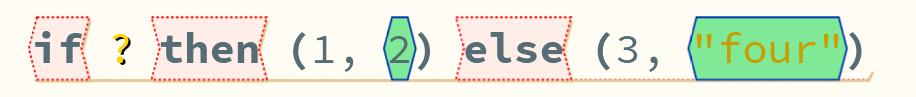
\includegraphics[width=1\textwidth]{Media/Figures/partially_inconsistent_branches}
\caption{Partially Inconsistent Branches}
\end{subfigure}$\qquad$
\begin{subfigure}{0.45\textwidth}
\centering

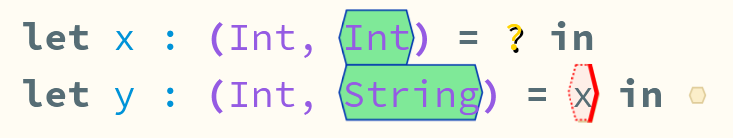
\includegraphics[width=1\textwidth]{Media/Figures/partially_inconsistent_expectations}
\caption{Partially Inconsistent Expectations}
\end{subfigure}

\caption{Error Slices}
\label{fig:ErrorSlice}
\end{figure}

Compound type inconsistencies necessarily differ at the outermost constructor (e.g., \code{List} vs \code{Int}), being the \textit{primary} cause of the error. Deeper inconsistencies are not those causing the type error. Therefore, we could extract only the slice on the outermost constructor. These minimised slices (\cref{fig:MinimisedSlice}) are significantly (avg. 3x) smaller than full combined slices (\cref{fig:TypeSlicingEffectiveness}). This ratio may grow with program complexity.\footnote{The dataset had few partially inconsistent cases, where the biggest savings occur.} This is now the default UI for type errors (with colours to distinguish the two parts).

\begin{figure}[h]
\centering
\begin{subfigure}{0.3\textwidth}
\centering

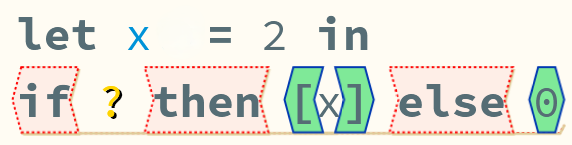
\includegraphics[width=1\textwidth]{Media/Figures/partially_inconsistent_compound}
\caption{Minimised Error Slice: Inner \code{Int} slice within list is omitted}
\end{subfigure}$\qquad\qquad$
\begin{subfigure}{0.3\textwidth}
\centering

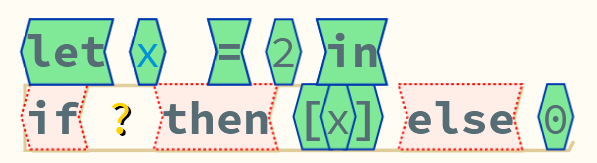
\includegraphics[width=1\textwidth]{Media/Figures/partially_inconsistent_compound_ordinary}
\caption{Ordinary Error Slice}
\end{subfigure}

\caption{Minimised Error Slices}
\label{fig:MinimisedSlice}
\end{figure}

\subsection{Structure Editing}\label{sec:StructureEditing}
Hazel uses a structure editor with an update calculus \cite{HazelStructureCalculus}, where statics are recalculated on edits, even cursor movement. While slice-based type checking is fast, it's less ideal for such interactive use in large programs.

Hazel ensures efficient edits\footnote{In constant time.} via a zipper data structure \cite{Zipper, OneHoleContext}. Extending this to the AST and typing info could enable edits to only locally update the type  information. However, some edits (e.g. adding a binding) can cause non-local, more extensive, type recalculation, but, these are rare. Such a system would require a major rewrite of Hazel's statics, with benefits beyond just type slicing.
  
\subsection{Static-Dynamic Error Correspondence}
\label{sec:ErrorCorrespondence}

A static type error will place a term inside a cast error during elaboration, which can be associated with a dynamic error whose cast error is dependent on (decomposed from, \cref{sec:CastDependence}) this original failed cast. This works well for \textit{inconsistent expectations} static type errors.

However, for inconsistent branches, no direct cast failure occurs until both are evaluated in a shared static context. The search might find such cases, but linking them back to the static error is harder. Still, since elaboration adds casts to each branch, these can be tracked with the error.\footnote{But we cannot assume the inconsistent branches caused the error; it might instead be the context using the value that is incorrect.}
  
\subsection{Categorising Programs Lacking Type Error Witnesses}
47 programs which timed out under the BDFS search procedure were manually inspected and classified as either:
\begin{itemize}
\item Witness Exists: BDFS failed to find an existing witness.
\item Dead Code: The error lies in unreachable code under all valid type instantiations, subdivided into:
\begin{itemize}
\item Pattern Cast Failure: Error within a pattern matching branch, making the branch unreachable. These are detectable by the extended pattern directed instantiation algorithm (\cref{sec:ExtendedPatternMatching}).\footnote{The inconsistent patterns would be attempted, and subsequently reduced to expression cast failures.}
\item Unbound Constructor: Attemping to match an unbound constructor. Also detectable with the extended instantiation.
\item Wildcards: Erroneous code bound to the inaccessible wildcard pattern: \code{let _ = ... in ...}.
\item Non-Trivial: Less easily detectable. One example exhibited this, infinitely recursing for all inputs.
\end{itemize}
\item Hazel Bugs: Unboxing bugs present in the main branch (excluded from the statistics).
\end{itemize}
\Cref{fig:FailureDistribution} shows this distribution and three (paraphrased) examples are given in \cref{fig:FailureExamples}. The full classification is in \texttt{failure-classification.txt}.

\begin{figure}[h]
\centering
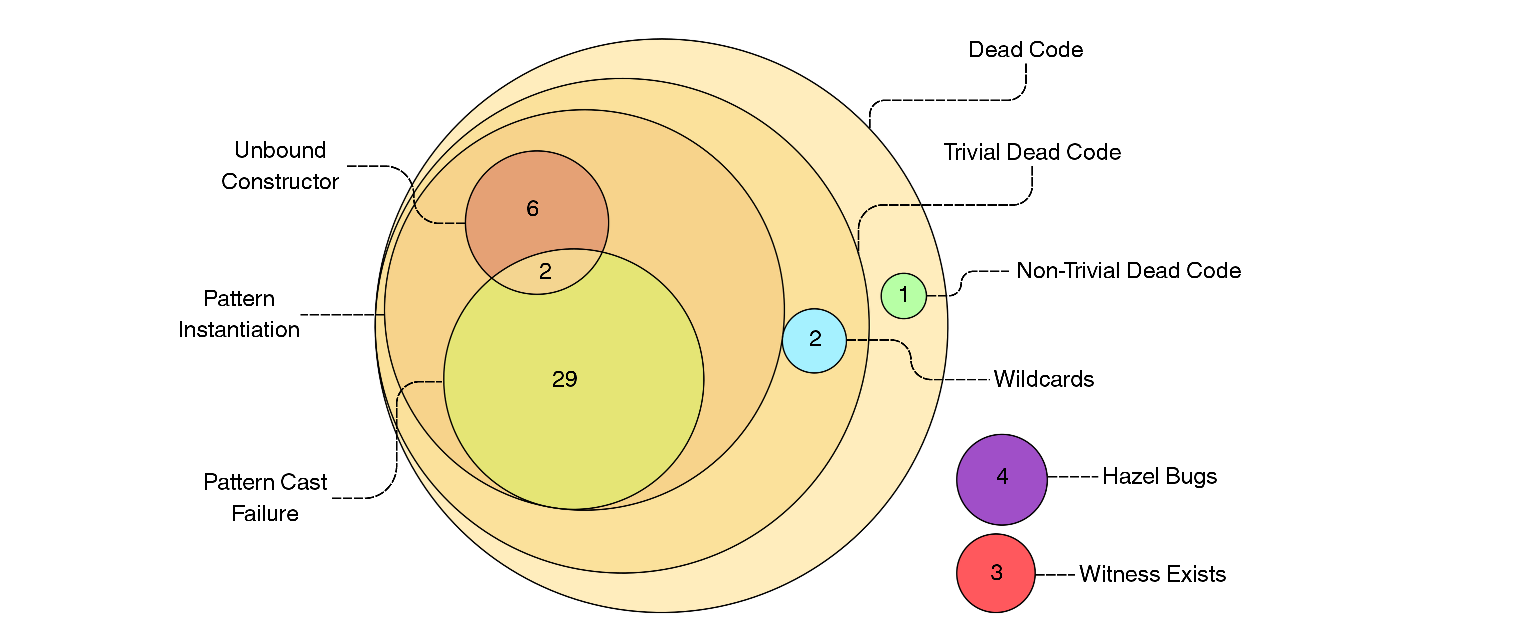
\includegraphics[width=1\textwidth]{Media/Figures/Failures}
\caption{Distribution of Failed Program Classes}
\label{fig:FailureDistribution}
\end{figure}

\begin{figure}
\centering
\begin{subfigure}{1\textwidth}
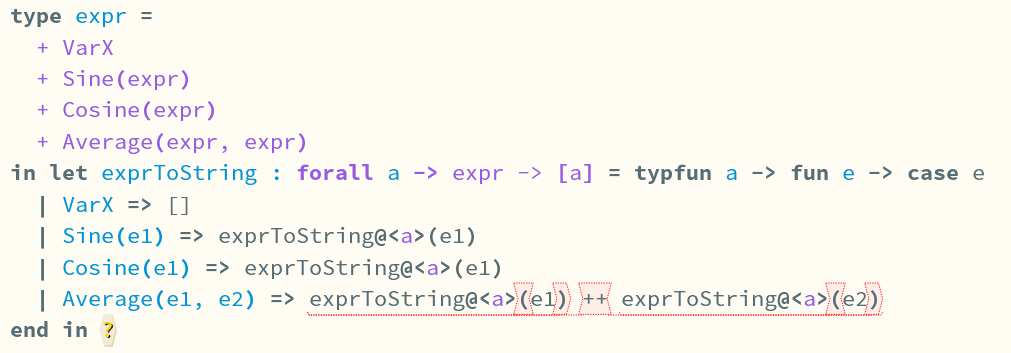
\includegraphics[width=1\textwidth]{Media/Figures/witness_exists}

Depth-first bias caused the procedure to try mostly permutations of \code{Sine(...)} and \code{Cosine(...)}. The error was on the \code{Average(...)} branch, not found within the time limit.
\caption{Witness Exists: prog2270.typed.hazel}
\end{subfigure}

\begin{subfigure}{1\textwidth}
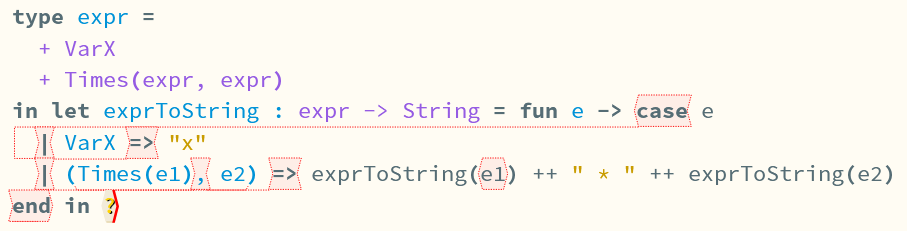
\includegraphics[width=0.8\textwidth]{Media/Figures/dead_code_pattern_instantiation}
A tuple pattern is used when an \code{expr} is expected. Instantiation only tries value of type \code{expr}. Further, another error exists inside this inaccessible branch.
\caption{Dead Code -- Wildcard: prog0080.typed.hazel}
\end{subfigure}

\begin{subfigure}{0.7\textwidth}
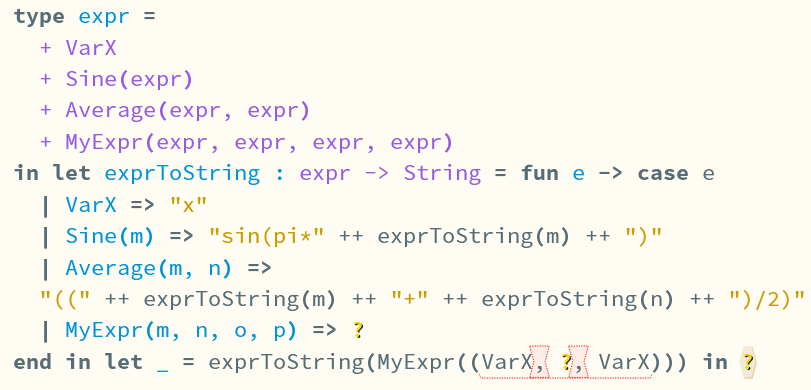
\includegraphics[width=1\textwidth]{Media/Figures/dead_code_wildcard}
Product arity inconsistency is present in inaccessible code bound to the wildcard pattern.
\caption{Dead Code -- Pattern Cast Failure: prog0339.typed.hazel}
\end{subfigure}
\caption{(Paraphrased) Failure Examples}
\label{fig:FailureExamples}
\end{figure}

\label{sec:SearchCategories}
\subsubsection{Non-Termination, Unfairness, and Search Order}
DFS is fast but prone to non-termination, giving it lesser coverage than BDFS (\cref{fig:PieChart}). If evaluation infinitely loops, so will DFS without exploring other instantiations. It is also unfair, it may never try some instantiations, e.g. instantiating \code{(}\dyn\code{, }\dyn\code{)} will yield \code{(0, 0)}, \code{(0, 1)}, etc., but never \code{(1, 0)} (\cref{fig:DFS}). This affected 10\% of cases.

To address this, BDFS, BFS, and IDFS were implemented, with BDFS performing best due to its preference for evaluation and low memory use (\cref{fig:SearchPerformance}).

\begin{figure}[H]
\centering
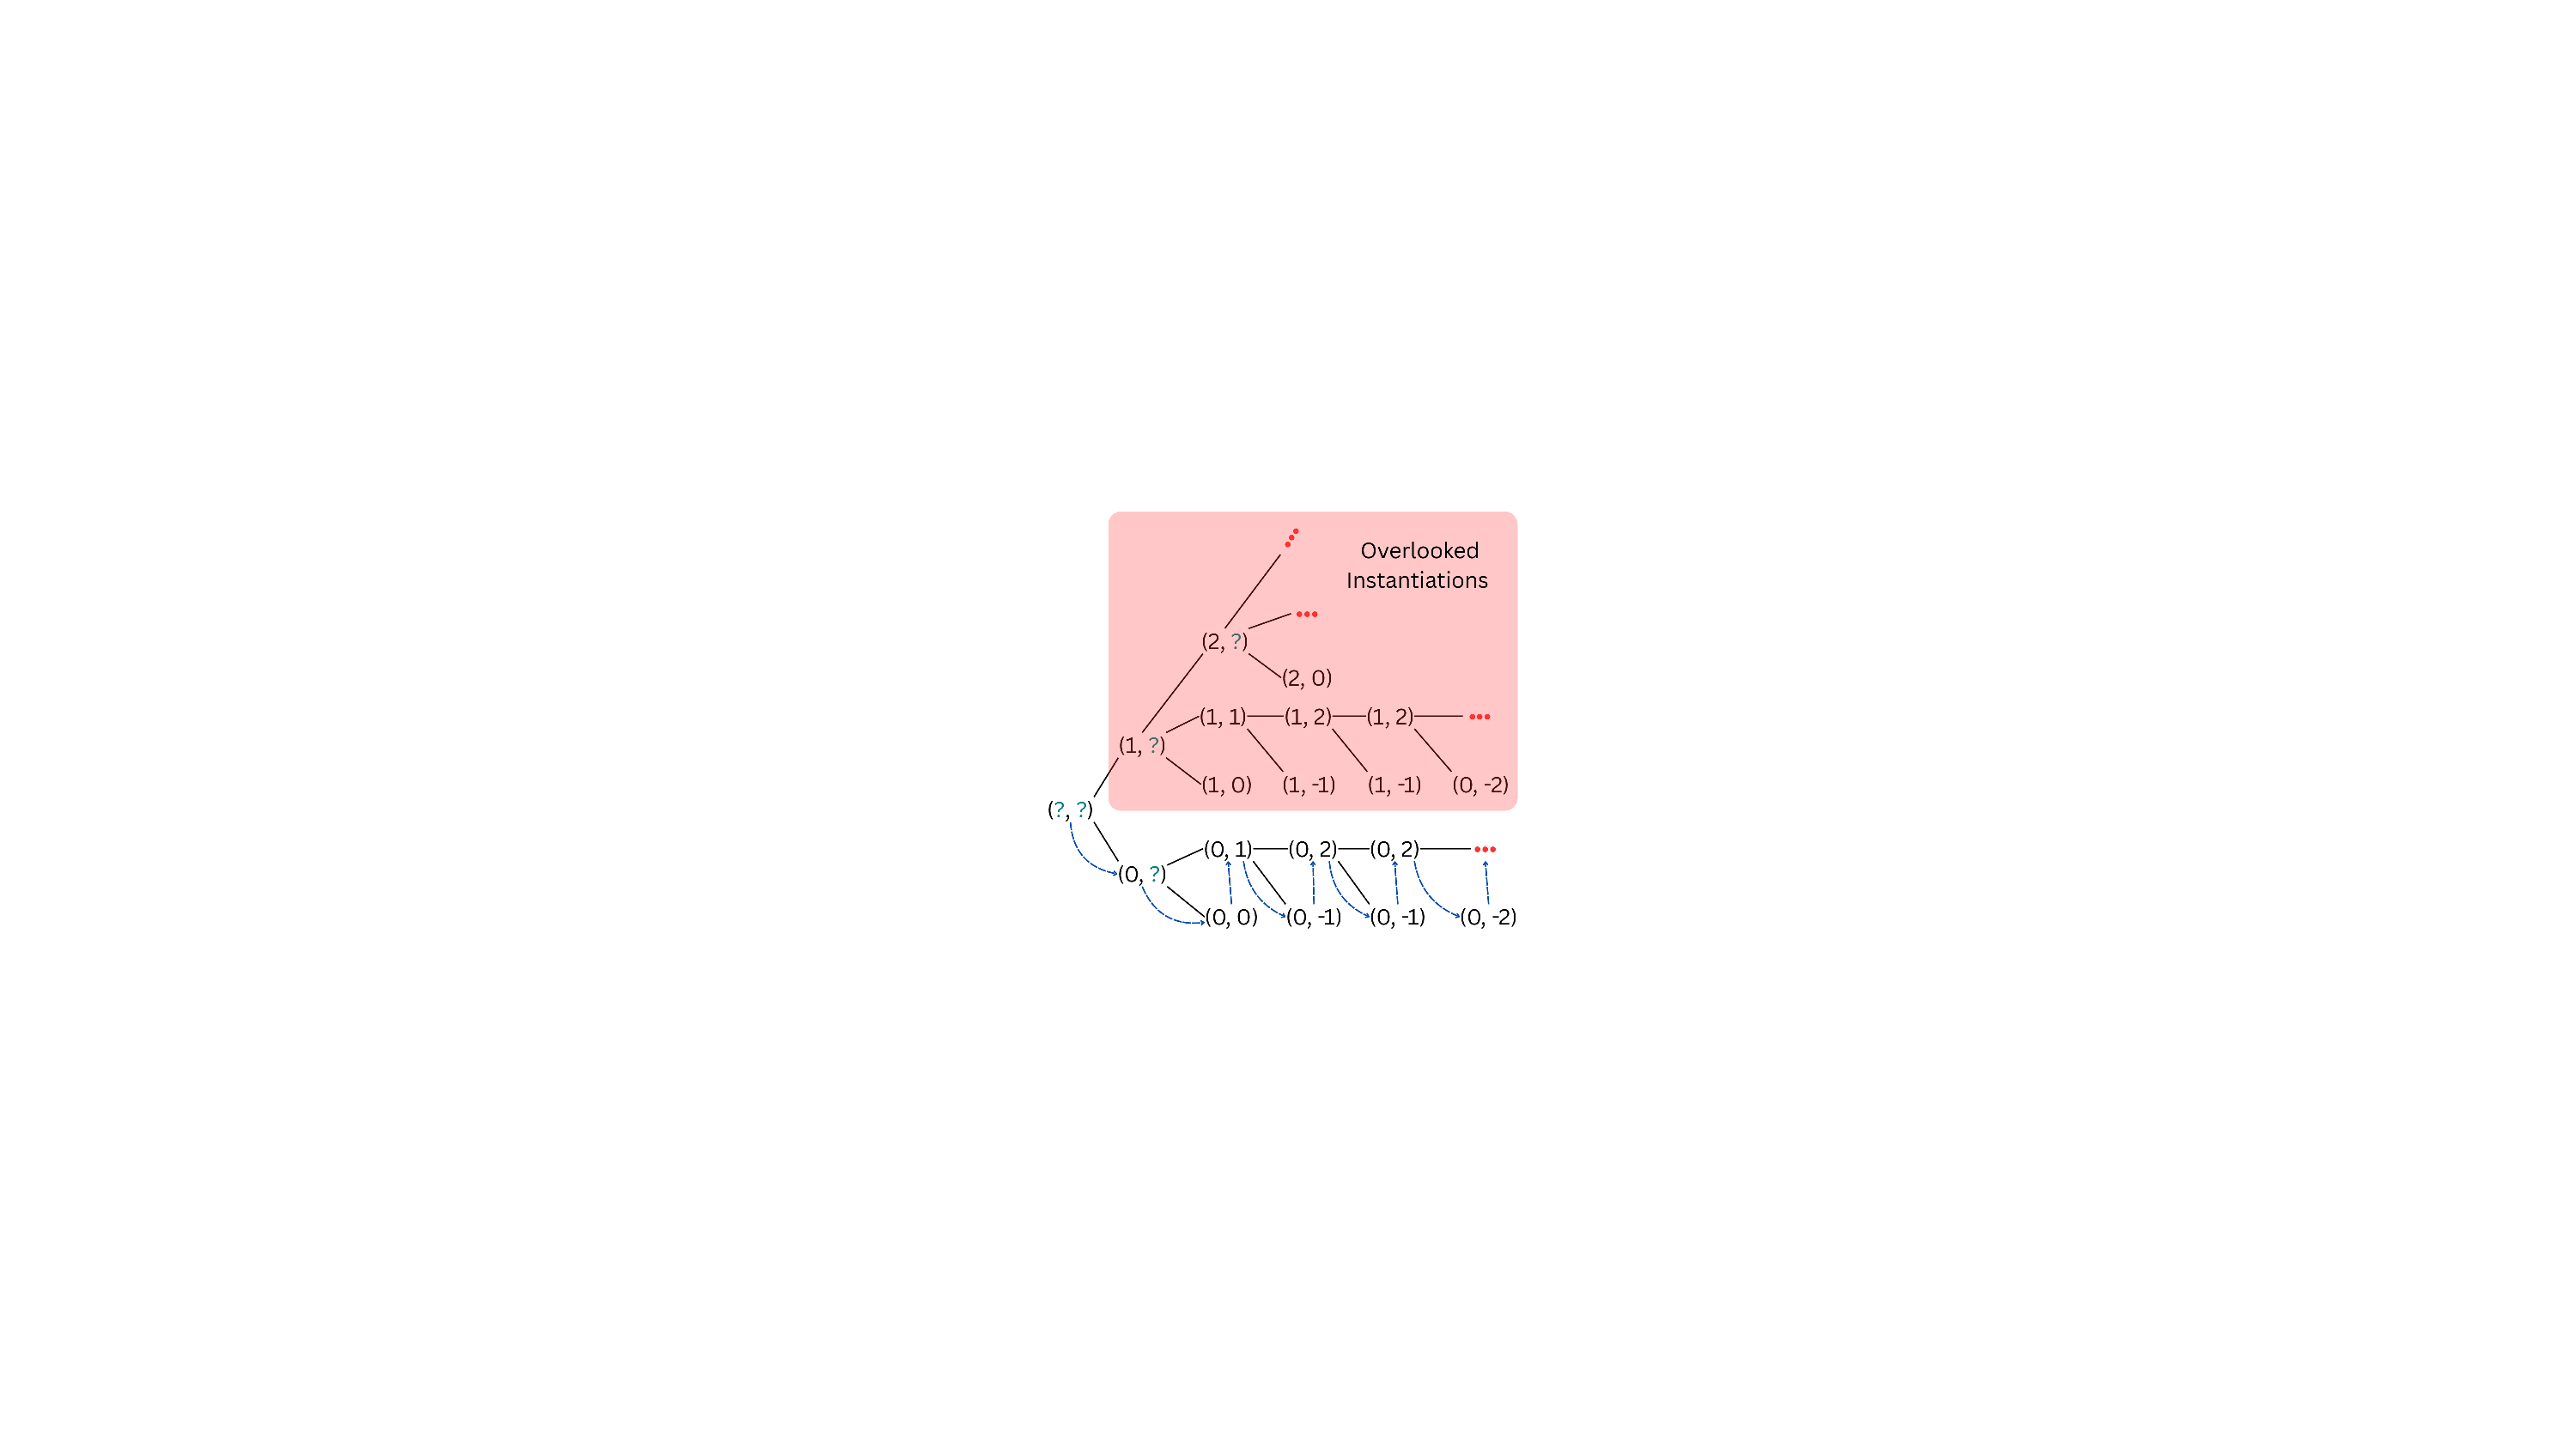
\includegraphics[width=1.25\textwidth, trim={15cm 10cm 10cm 10cm},clip]{Media/Figures/DFS}
\caption{Non-exhaustive Instantiations in DFS}
\label{fig:DFS}
\end{figure}
BFS and IDFS would do significantly better if evaluation were less frequently wrapped deeper in the search tree (reducing the \textit{cost} of evaluation).  Choosing how frequently to wrap evaluation is a delicate balancing act between finding errors deeper in evaluation vs. attempting more instantiations.

\subsubsection{Dead Code \& Nested Errors}

Dead code caused most time outs for the search procedure using BDFS. Errors within dead code cannot have a witness as they are not dynamically reachable. Therefore, dead code analysis will reduce timeouts.

Additionally, code can become dead due to errors. 12 (32\%) of the dead code classified had a nested error within a branch, unreachable due to a pattern error\footnote{Unbound constructor or inconsistent expectations.} within the branch pattern. Even if witnesses are found for these branch errors, the nested errors remain hidden.

\subsubsection{Dynamically Safe Code}
Some static errors is inherently dynamically safe, having no witness, e.g. \code{if true then 0 else "str"}. The search procedure often proves this by running out of instantiations: BDFS proved no witness 12\% of the time. 

However, in general, safe code may lead to non-terminating searches, endlessly generating witnesses. So, a timeout does not necessarily imply a witness was found, or that none exist.

\subsubsection{Cast Laziness}\label{sec:EvalCastLaziness}
Hazel treats casts lazily, only pushing casts on compound data to their elements upon usage. The instantiation procedure is therefore unable to instantiate parts of compound data until it is de-structured: for example, extracting the first element of a tuple. Further, Hazel does not detect cast errors between non-ground compound types (e.g. \code{[Int]} and \code{[String]}). Therefore, type inconsistencies between such types will not be found by the search procedure. These errors are less common, in the search corpus there were \textit{no} programs exhibiting this.

Hazel treats casts lazily, deferring cast transitions on compound data until their elements are used (e.g., tuple elements). Therefore, these elements cannot be instantiated until the data is deconstructed. Further, Hazel cannot detect cast errors between non-ground compound types (e.g., \code{[Int]} vs \code{[String]}), therefore if such compound type's elements are unused, the errors cannot be witnessed. These errors are uncommon, none appeared in the search corpus.

Addressing this would require eager cast semantics, as has been previously explored for dynamic and gradual type systems \cite{EagerCasts, GradualEagerCasts}.\footnote{Often referred to as coercions.} Alternatively, more sophisticated instantiation could track hole types of compound data elements using the outer casts, but this still needs eager error checks.

Eager casts would catch dynamic errors earlier. For example, \cref{fig:LazyCastError} shows a cast inconsistency undetected (by lazy casts) at runtime until the tuple element is accessed.
\begin{figure}[h]
\centering
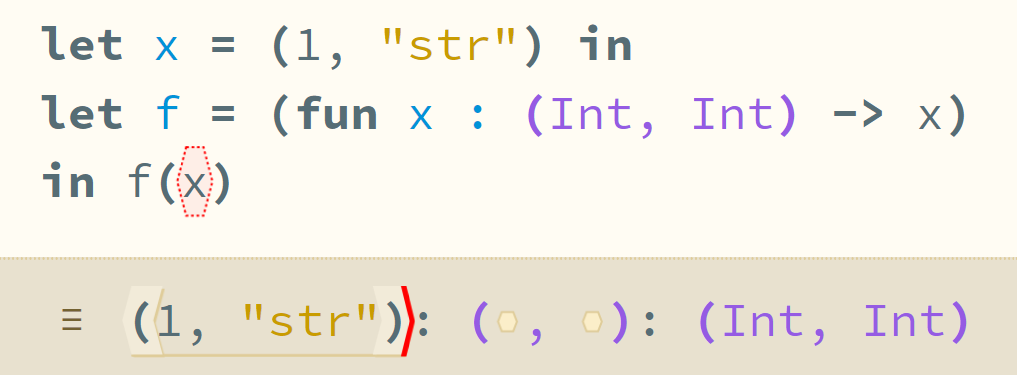
\includegraphics[width=0.55\textwidth]{Media/Figures/cast_laziness_no_error}
\caption{Inconsistent Lazy Casts: No Cast Failure}
\label{fig:LazyCastError}
\end{figure}

\subsubsection{Combinatorial Explosion}
When multiple holes are involved when searching, the search space increases exponentially.

Combinatorial explosion especially impacts IDFS and BFS, who prioritise instantiation over evaluation. This leads to high memory use and hinders evaluation from progressing far enough to detect errors, even when valid witnesses have been instantiated.

Further, some errors only arise on very specific inputs, e.g. \code{(23, 31)} and \code{(31, 23)} in \cref{fig:SpecificInstantiations}. Directing instantiation to maximise code coverage earlier could find such errors attempting fewer instantiations.
\begin{figure}\centering
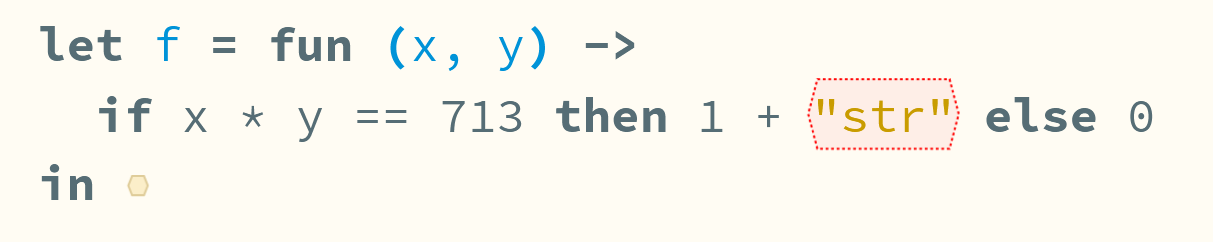
\includegraphics[width=0.6\textwidth]{Media/Figures/very_specific_error}
\caption{Witness Requiring Very Specific Instantiations}
\label{fig:SpecificInstantiations}
\end{figure}

\subsection{Improving Code Coverage}
\label{sec:EvalHoleInstantiation}
Of the program classes lacking type error witnesses (\cref{sec:SearchCategories}), only 3 had concrete witnesses missed, each due to instantiations happening not to execute the erroneous branch.

These often require specific, interdependent inputs, so are less likely to instantiate. These errors are harder for programmers to detect or understand. Understanding the error might require recognizing input interdependencies.

Intelligently directing hole instantiations to better cover the code would help. Symbolic execution and program test generation are well-researched areas having explored this, producing constraint solvers and translation to theories for SMT solvers.

A pattern-directed instantiation as described in \cref{sec:ExtendedPatternMatching} would discover 2 of the 3 missed witnesses by BDFS. Extended symbolic execution could deal with (\code{Int} and \code{Float}) inequalities and conditionals.

Still, BDFS retains a very high coverage over the search procedure (97\%), excluding dead code.

\section{Holistic Evaluation}
\label{sec:HolisticEvaluation}

This section considers a number of examples of ill-typed Hazel programs, \textit{holistically} and \textit{qualitatively} evaluating how a user might use the three features and the existing bidirectional type error localisation \cite{MarkedLocalisation} to debug the errors. 


\subsection{Interaction with Existing Hazel Type Error Localisation}
Hazel has three error types addressed by this project:\footnote{Other errors: syntax errors, unbound variables, label errors etc. are out of scope} \textit{inconsistent expectations} (analytic and synthetic types are inconsistent), \textit{inconsistent branches }(branches or list element types are inconsistent), and \textit{inexhaustive matches}. 

\Cref{sec:ErrorCorrespondence} showed how witnesses can be associated to inconsistency errors. Generating examples for inexhaustive match statements was not a core aim, but witnesses for this can be found. Static generation of such examples is already a (mostly)\footnote{Data abstraction can cause issues: for example Views \cite{Views} and Active Patterns {\cite{ActivePatterns}}. Hazel is implementing modules, but yet to consider pattern matching on abstract data.} solved problem \cite{PatternMatchingWarnings}, and is under development for Hazel. Pattern matrices are preferable (faster), and would aid directing hole instantiation (\cref{sec:EvalHoleInstantiation}).

The situations where a programmer does not understand why an error occurs generally arise due to a \textit{misunderstanding} about the types of the code. In which case, existing error localisation is not so useful as the location of an error is determined while making \textit{differing assumptions} about the types than the programmer. Type slicing, along with the context inspector (which shows the type, term, and describes the error of a selected expression: \cref{fig:ContextInspector}), can help the programmer understand which assumptions the type system is making and \textit{why} it is. 

When errors arise from the programmer misunderstanding the program types, error localisation can be inaccurate (due to assuming different types to the programmer's expectations). The context inspector (\cref{fig:ContextInspector}) clarifies what assumptions the system makes while slicing and witnesses can explain \textit{why}.

\begin{figure}[h]\centering
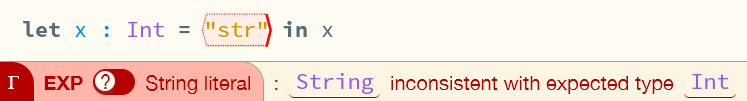
\includegraphics[width=0.7\textwidth]{Media/Figures/context_inspector}
\caption{Selected Static Error described by Hazel Context Inspector}
\label{fig:ContextInspector}
\end{figure}

When the programmer and system agree on the types, bidirectional typing generally localises the error(s) well \cite{BidirectionalTypes, MarkedLocalisation}. However, there is not always enough static information to even recognise errors. The search procedure tests such code for such type errors automatically. 

Alternatively, annotations can be added to locate the errors. However, this is time-consuming, many annotations may be required to detect the error statically. It can make sense to use the search procedure to check for errors more quickly. \Cref{fig:HalfAnnotated} shows a mostly annotated map function, still not providing sufficient type information to detect the error statically.


\begin{figure}[H]
\centering
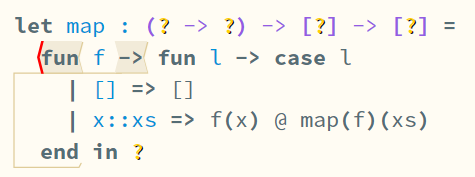
\includegraphics[width=0.5\textwidth]{Media/Figures/partial_annotations}
\caption{Partially Annotated Program misses Error: Concatenation (\code{@}) used instead of cons (\code{::})}
\label{fig:HalfAnnotated}
\end{figure}

\subsection{Examples}
\label{sec:EvalExamples}
Returning to the map example, when fully annotated a static error can located at \code{f(x)} which has type \code{Int} but expects \code{[Int]}. The error slice shows (in pink) why \code{Int} is synthesised (due to input \code{f} being annotated \code{Int -> Int} and applied) and (in blue) why a list\footnote{A full analysis slice would also include the full \code{[Int]} annotation. But the inconsistency arises from the list part.} is expected (being an argument of list concatenation). See \cref{fig:MapExample}.

\begin{figure}[h]
\centering
\begin{subfigure}{0.49\textwidth}
\centering
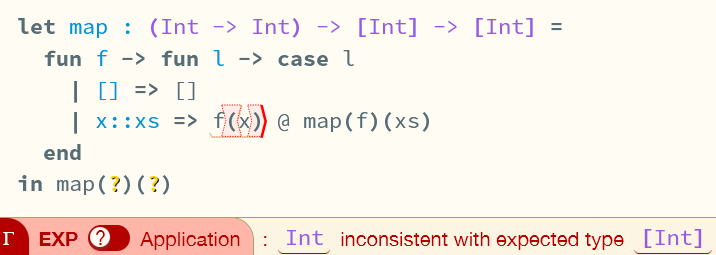
\includegraphics[width=1\textwidth]{Media/Figures/map_example}
\caption{Error}
\end{subfigure}
\begin{subfigure}{0.49\textwidth}
\centering
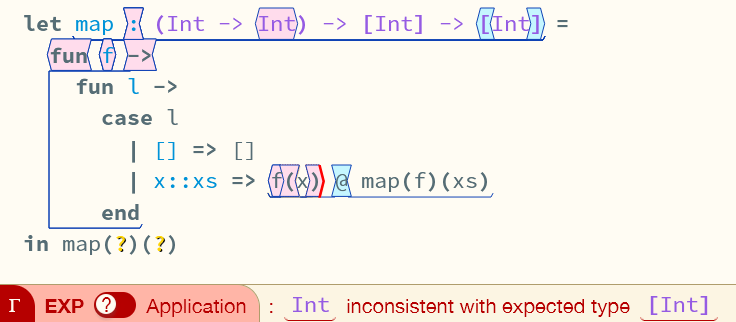
\includegraphics[width=1\textwidth]{Media/Figures/map_example_sliced}
\caption{With Error Slice}
\end{subfigure}
\caption{Example: Type Slice of Inconsistent Expectations}
\label{fig:MapExample}
\end{figure}

Similarly, error slicing works for inconsistent branches: \cref{fig:InconsistentBranchesExample} demonstrates a somewhat more complex inconsistency involving non-local bindings. With \textit{minimal} error slices highlighting only the bindings, and conflicting addition and string concatenation operators.

\begin{figure}[h]
\centering
\begin{subfigure}{0.49\textwidth}
\centering
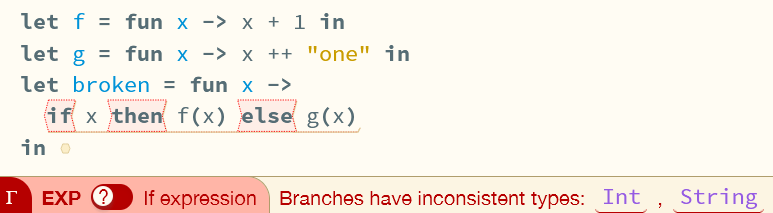
\includegraphics[width=1\textwidth]{Media/Figures/inconsistent_branches_example}
\caption{Error}
\end{subfigure}
\begin{subfigure}{0.49\textwidth}
\centering
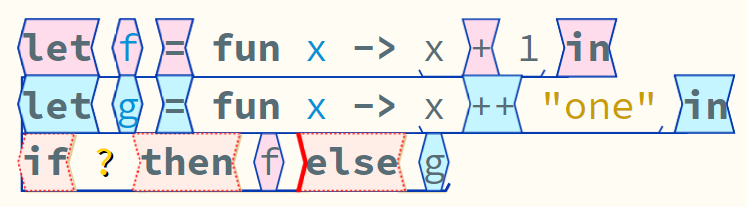
\includegraphics[width=1\textwidth]{Media/Figures/inconsistent_branches_example_sliced}
\caption{With Error Slice}
\end{subfigure}
\caption{Example: Type Slice of Inconsistent Branches}
\label{fig:InconsistentBranchesExample}
\end{figure}

Not every static type error slice is concise or obvious. I demonstrate this by returning to the example from the introduction (\cref{fig:ConcatError}). The user mistakes list cons \code{::} for list concatenation \code{@}. The type slice does highlight the \code{::} and annotation enforcing \code{x} as an \code{Int}, but they might not understand why if they still expect \code{::} to perform concatenation. Additionally, there is considerable noise from the synthesis slice distracting from this. A type witness demonstrates concretely how this program goes wrong: that the lists are not being concatenated. The user can cycle through increasingly larger witnesses\footnote{Looking at larger witnesses can be useful to spot pattern with what is happening overall, i.e. that the lists are being consed, not concatenated.}. Finally, the cast slice to \code{Int} concisely retrieves relevant part of the original type slice.
\begin{figure}[H]
\centering
\begin{subfigure}{0.49\textwidth}
\centering
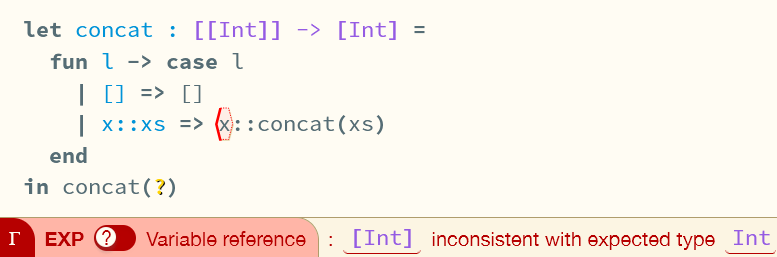
\includegraphics[width=1\textwidth]{Media/Figures/concat_error}
\caption{Error: Mistaken Cons for Concat}
\end{subfigure}
\begin{subfigure}{0.49\textwidth}
\centering
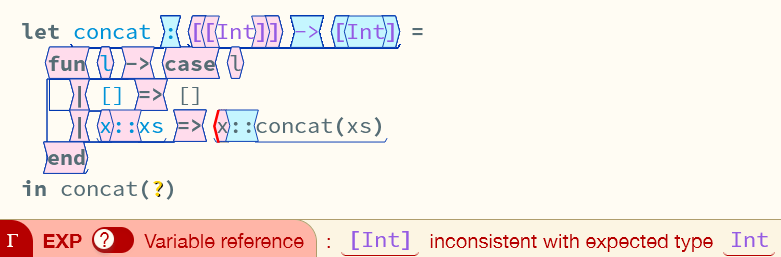
\includegraphics[width=1\textwidth]{Media/Figures/concat_error_type_slice}
\caption{Verbose Type Slice}
\end{subfigure}
\begin{subfigure}{0.49\textwidth}
\centering
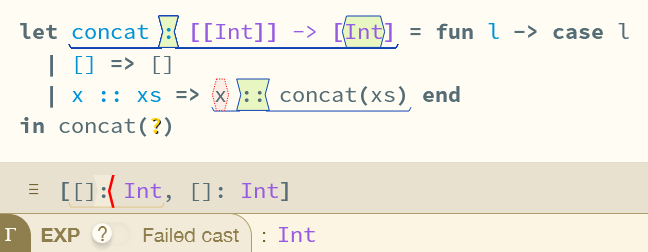
\includegraphics[width=1\textwidth]{Media/Figures/concat_error_cast_slice}
\caption{A Witness \code{([[], []])} leading to concise Cast Slice}
\end{subfigure}
\begin{subfigure}{0.49\textwidth}
\centering
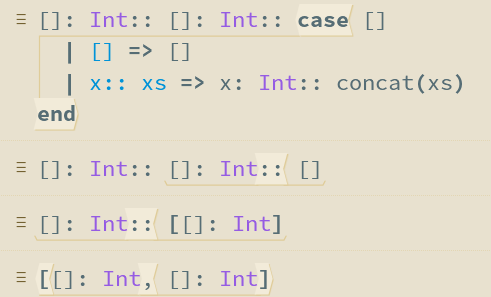
\includegraphics[width=1\textwidth]{Media/Figures/concat_error_trace}
\caption{Last 3 steps in witness trace: Shows \code{::} being List Cons}
\end{subfigure}
\caption{Example: Witnesses and Cast Slice more Understandable than Type Slice}
\label{fig:ConcatError}
\end{figure}
Another, more subtle, example is confusing curried and non-curried functions: \cref{fig:TastyCurry} implements a \code{fold} function taking curried functions, but tries to apply an uncurried \code{add} function to sum int lists. This example shows how a single error can result in \textit{multiple} cast errors, each having a more concise slice explaining them. See how the type slice had two inconsistencies (in both the argument and return type of add), which were then separated into two different cast errors: \code{add} expected it's argument to be a tuple, \code{fold} expected the result of \code{add} to be a function.

\begin{figure}[h]
\begin{subfigure}{0.49\textwidth}
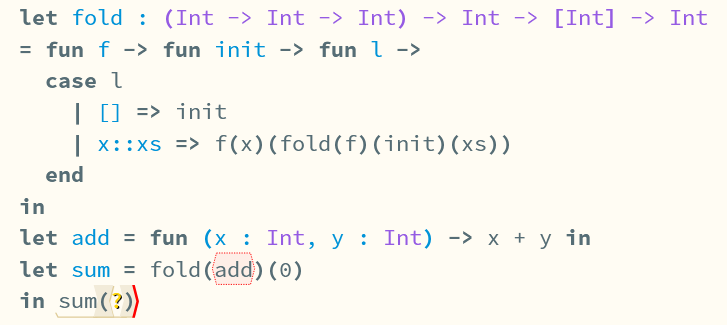
\includegraphics[width=1\textwidth]{Media/Figures/curries}
\caption{Confused uncurried for curried \code{add}}
\end{subfigure}
\begin{subfigure}{0.49\textwidth}
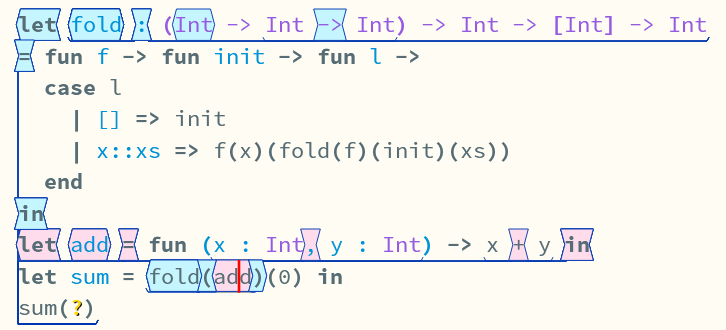
\includegraphics[width=1\textwidth]{Media/Figures/curries_type_slice}
\caption{Somewhat Verbose Type Slice}
\end{subfigure}
\begin{subfigure}{0.49\textwidth}
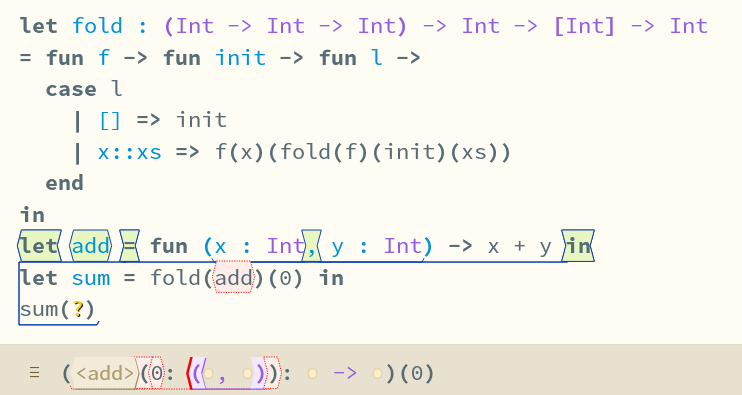
\includegraphics[width=1\textwidth]{Media/Figures/curries_expects_tuple}
\caption{Witness (\code{[0]}) expects input to \code{add} to be a tuple}
\end{subfigure}
\begin{subfigure}{0.49\textwidth}
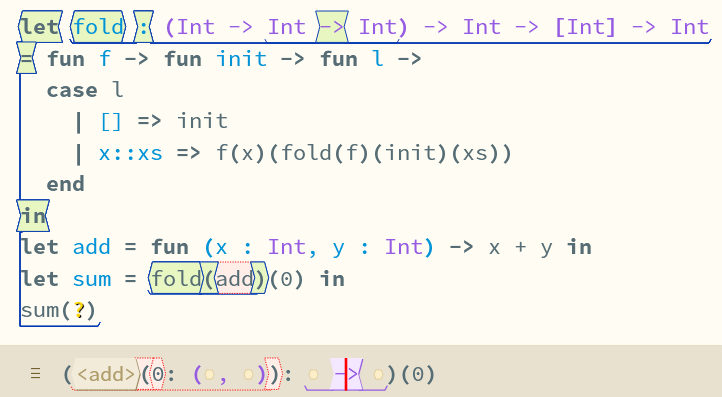
\includegraphics[width=1\textwidth]{Media/Figures/curries_expects_function}
\caption{Witness (\code{[0]}) expects output of \code{add(0)} to be a function}
\end{subfigure}
\caption{Example: Subtle Currying Error}
\label{fig:TastyCurry}
\end{figure}

Finally, when code is dynamic, errors might not be statically found, and type slices have less information to work with. \Cref{fig:DynamicExample} considers finding a simple error in a dynamic function. Cast slicing still works even without type annotations, allowing errors to blame regions of the source code.
\begin{figure}[h]
\centering
\begin{subfigure}{0.45\textwidth}
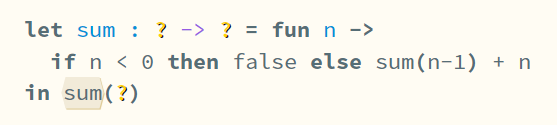
\includegraphics[width=1\textwidth]{Media/Figures/dynamic_code_error}
\caption{Error}
\end{subfigure}
\begin{subfigure}{0.45\textwidth}
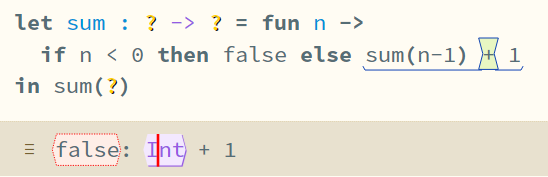
\includegraphics[width=1\textwidth]{Media/Figures/dynamic_code_error_cast_slice}
\caption{Automated witness found with cast slice blaming \code{+} operator}
\end{subfigure}
\caption{Example: Searching for Error in Dynamic Code}
\label{fig:DynamicExample}
\end{figure}


\subsection{Usability Improvements}\label{sec:UIImprovements}
As designing an intuitive UI was not a core goal, using the features can feel awkward or unintuitive. Below are proposed improvements, which the architecture of both Hazel and the new features can easily support:

\begin{itemize}
\item Display type slices only \textit{upon request} using the Hazel context inspector, showing the \textit{analysing} and \textit{synthesising} types of the selected expression, see \cref{fig:ContextInspector}.
\item Allow users to deconstruct type slices to query specific parts, e.g. select the just the sub-slice explaining the \textit{return type} of a function or just the function arrow part. This could be done by selecting the type parts in the context inspector.
This interaction would help users really understand how code comes together to define it's types.
\item Visualise graphs of cast dependencies, showing the \textit{execution} context leading to a cast error, summarising more concisely than full evaluation traces.
\item Provide a UI for the search procedure's execution traces and instantiations, integrated with Hazel's trace visualiser. This could include trace compression for better readability (e.g., skipping irrelevant function calls).
\item Implement key bindings to cycle through indeterminate evaluation paths more quickly.
\end{itemize}